% Author         : Manuel Lippert
% Version        : 1.1
% Created on     : 11.06.2023
% Last Edited on : 11.06.2023

%%%%%%%%%%%%%%%%%%%%%%%%%%%%%%%%%%%%%%%%%%%%%%%%%%%%%%%%%%%%%%%%%%%%%%%%%%%
%                    !!! Compile with LuaLaTex !!!
%%%%%%%%%%%%%%%%%%%%%%%%%%%%%%%%%%%%%%%%%%%%%%%%%%%%%%%%%%%%%%%%%%%%%%%%%%%

\documentclass[compress,aspectratio=43]{beamer}

%--------------------------------------------------------------------------
% Theme
%--------------------------------------------------------------------------

\usepackage{theme/beamerthemefancy}
\usetheme{fancy}

\usepackage{theme/dtklogos} % must be loaded after theme

%--------------------------------------------------------------------------
% Common packages
%--------------------------------------------------------------------------

\usepackage[ngerman]{babel}
\usepackage{graphicx}
\usepackage{multicol}
\usepackage{multimedia}
\usepackage{media9}
\usepackage{hyperref}
\usepackage{tabularx}
\usepackage{tikz}
\usepackage{booktabs}
\usepackage{soul}

%--------------------------------------------------------------------------
% Functions, Graphics, Tikz, Underlines
%--------------------------------------------------------------------------

\usetikzlibrary{mindmap,backgrounds}
\graphicspath{{../pictures/}}

\newcommand{\tabitem}{~~\llap{\textbullet}~~}
\newcommand{\vect}[1]{\boldsymbol{\mathbf{#1}}}

\setul{0.3ex}{0.2ex}

\makeatletter 
\let\UL\ul 
\renewcommand\ul{
	\let\set@color\beamerorig@set@color 
	\let\reset@color\beamerorig@reset@color 
	\UL} 
\makeatother

%--------------------------------------------------------------------------
% Document
%--------------------------------------------------------------------------

\title{Turbulenzen in Plasma}
\subtitle{Beispiel anhand von Plasma im Tokamak Reaktor}
\author{Manuel Lippert}
\institute{Physik (Master of Science)}

\begin{document}

	\maketitle

	\begin{frame}{Gliederung}
		\tableofcontents[hideallsubsections]
	\end{frame}
	
	\centering

	\section{Magnetohydrodynamische (MHD) Gleichungen}
	%\subsection{Magnetohydrodynamische Gleichungen}
	%\begin{frame}
	%	\frametitle{Magnetohydrodynamische Gleichungen}
	%	\begin{gather*}
	%		\begin{aligned}
	%			\partial_t \rho + \nabla \cdot (\rho \vect{v}) &= 0 \\
	%			\rho \partial_t \vect{v} + \rho (\vect{v} \cdot \nabla) \vect{v} + \nabla p &= \frac{\vect{J} \times \vect{B}}{c} + \rho \vect{g} + \vect{F} \\
	%			\nabla \times \vect{B} &= \frac{4 \pi}{c} \vect{J} \\
	%			\nabla \times \vect{E} &= -\frac{1}{c}\partial_t\vect{B} \\
	%			\nabla \cdot \vect{B} &= 0 \\
	%			\vect{J} &= \sigma \left(\vect{E} + \frac{\vect{v} \times \vect{B}}{c}\right)
	%		\end{aligned}
	%	\end{gather*}
	%\end{frame}

	\begin{frame}
		\frametitle{Magnetohydrodynamische (MHD) Gleichungen}
		\begingroup
			\setbeamercolor{block title}{bg=Sec3Dark}
			\setbeamercolor{block body}{bg=Sec3}
			\begin{block}{Kontinuitätsgleichung}
				\centering
				$\partial_t \rho + \nabla \cdot (\rho \vect{v}) = 0$
			\end{block}
		\endgroup
		\begingroup
			\setbeamercolor{block title}{bg=Sec2CompDark}
			\setbeamercolor{block body}{bg=Sec2Comp}
			\begin{block}{Navier-Stokes Gleichung}
				\centering
				$\rho \partial_t \vect{v} + \rho (\vect{v} \cdot \nabla) \vect{v} = - \nabla p + \frac{\vect{J} \times \vect{B}}{c} + \rho \vect{g} + \vect{F}$
			\end{block}
		\endgroup
		\begingroup
			\setbeamercolor{block title}{bg=Sec1Dark}
			\setbeamercolor{block body}{bg=Sec1}
			\begin{block}{Maxwell Gleichungen}
				\centering
				\begin{tabular}{l l}
					$\nabla \cdot \vect{B} = 0$ & $\nabla \times \vect{B} = \frac{4 \pi}{c} \vect{J}$ \\[0.3cm]
					$\vect{J} = \sigma \left(\vect{E} + \frac{\vect{v} \times \vect{B}}{c}\right)$ & $\nabla \times \vect{E} = -\frac{1}{c}\partial_t\vect{B}$ \\
				\end{tabular}
			\end{block}
		\endgroup
	\end{frame}
	\begin{frame}
		\frametitle{Beschreibung von Plasma im Tokamak Reaktor}
		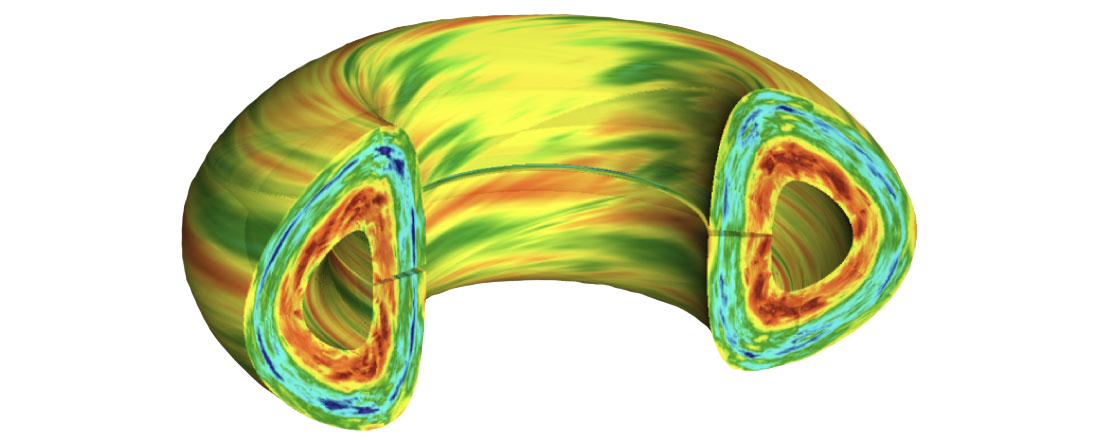
\includegraphics[scale = 1]{Presentation/Zonal_Flow.PNG}
		\begin{alertblock}{Achtung Instabilität am Plasmarand!}
			\centering
			Ionen Temperaturgradient Instabilität $\approx$ Rayleigh-Taylor Instabilität
		\end{alertblock}
	\end{frame}

	\section{Ionen Temperaturgradient (ITG) Instabilität}
	\begin{frame}
		\frametitle{ITG Instabilität am Plasmarand}
		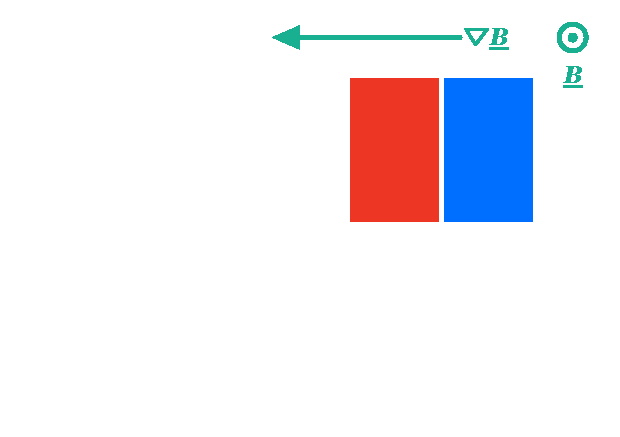
\includegraphics[scale=0.8]{Presentation/ITG_Instability_00.pdf}
	\end{frame}
	\begin{frame}
		\frametitle{ITG Instabilität am Plasmarand}
		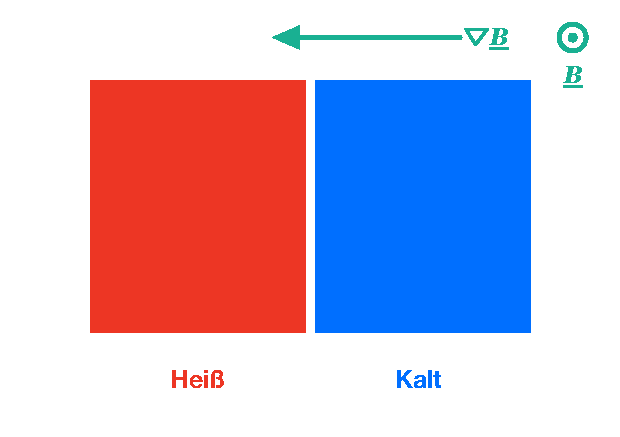
\includegraphics[scale=0.8]{Presentation/ITG_Instability_01.pdf}
	\end{frame}
	\begin{frame}
		\frametitle{ITG Instabilität am Plasmarand}
		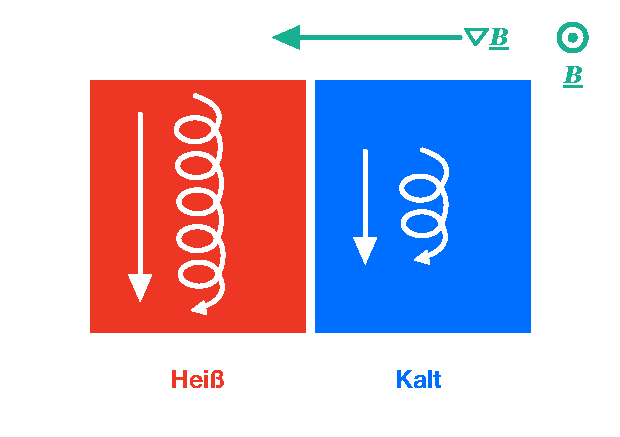
\includegraphics[scale=0.8]{Presentation/ITG_Instability_02.pdf}
	\end{frame}
	\begin{frame}
		\frametitle{ITG Instabilität am Plasmarand}
		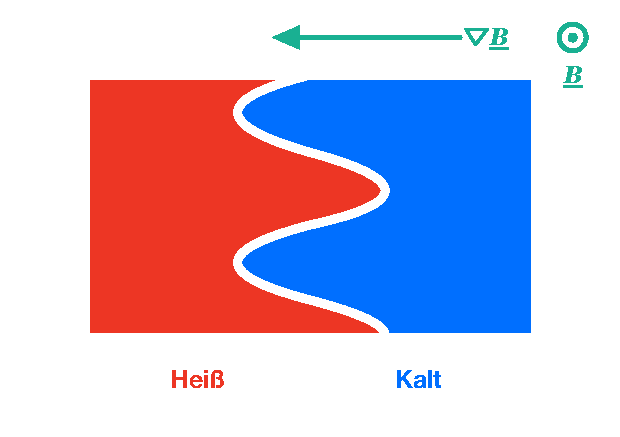
\includegraphics[scale=0.8]{Presentation/ITG_Instability_03.pdf}
	\end{frame}
	\begin{frame}
		\frametitle{ITG Instabilität am Plasmarand}
		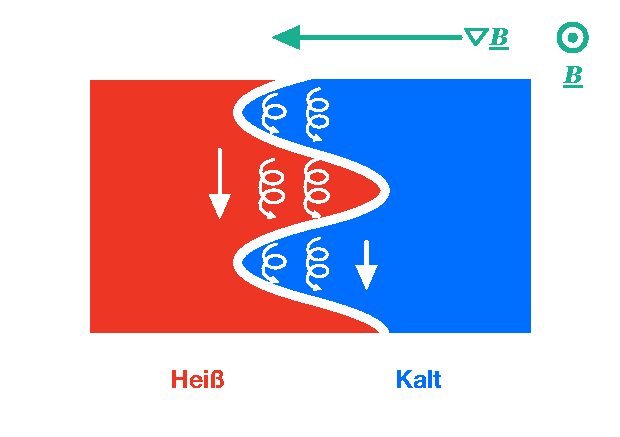
\includegraphics[scale=0.8]{Presentation/ITG_Instability_04.pdf}
	\end{frame}
	\begin{frame}
		\frametitle{ITG Instabilität am Plasmarand}
		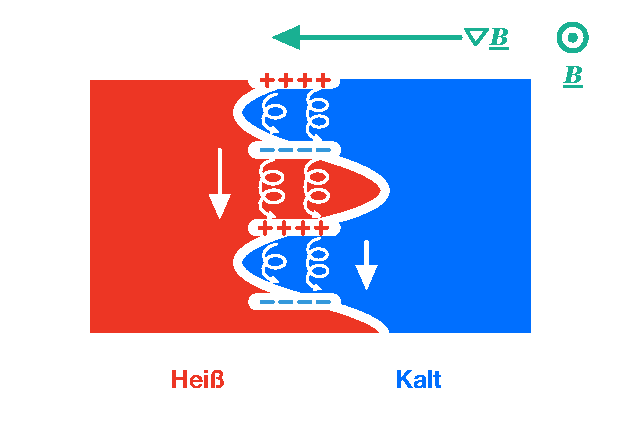
\includegraphics[scale=0.8]{Presentation/ITG_Instability_05.pdf}
	\end{frame}
	\begin{frame}
		\frametitle{ITG Instabilität am Plasmarand}
		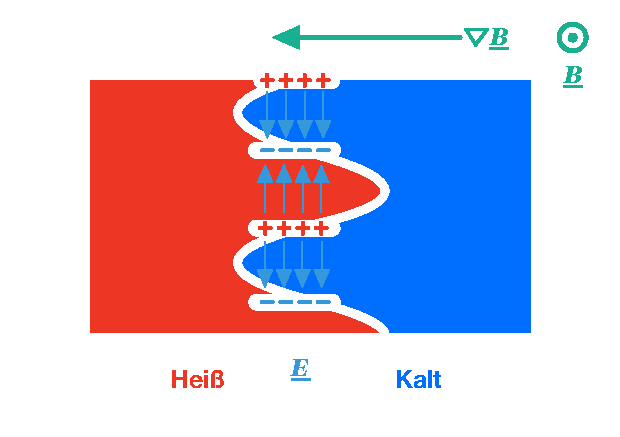
\includegraphics[scale=0.8]{Presentation/ITG_Instability_06.pdf}
	\end{frame}
	\begin{frame}
		\frametitle{ITG Instabilität am Plasmarand}
		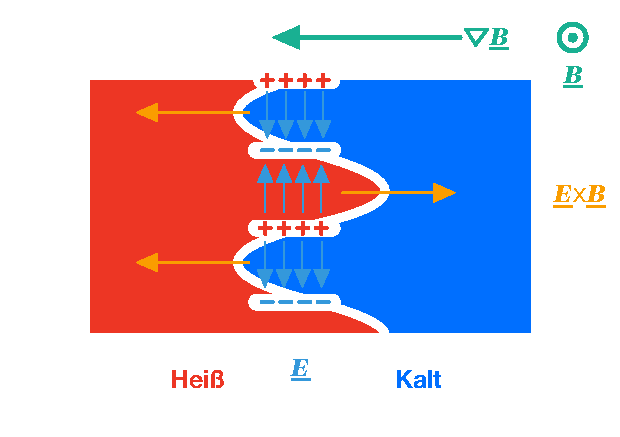
\includegraphics[scale=0.8]{Presentation/ITG_Instability_07.pdf}
	\end{frame}
	\begin{frame}
		\frametitle{ITG Instabilität am Plasmarand}
		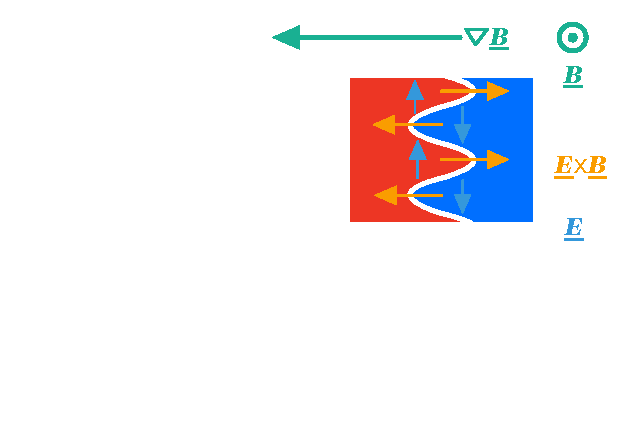
\includegraphics[scale=0.8]{Presentation/ITG_Instability_08.pdf}
	\end{frame}
	\begin{frame}
		\frametitle{ITG Instabilität am Plasmarand}
		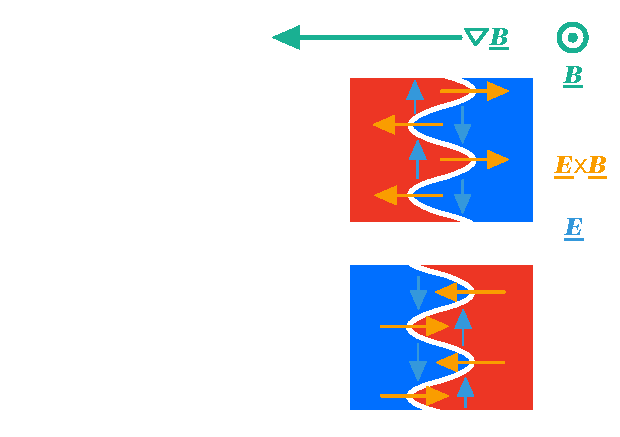
\includegraphics[scale=0.8]{Presentation/ITG_Instability_09.pdf}
	\end{frame}
	\begin{frame}
		\frametitle{ITG Instabilität am Plasmarand}
		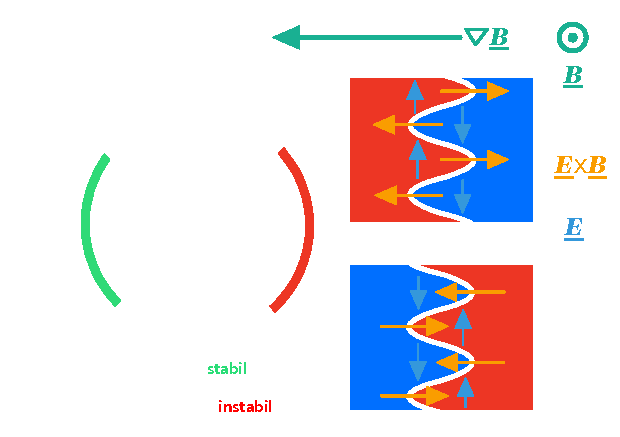
\includegraphics[scale=0.8]{Presentation/ITG_Instability_10.pdf}
	\end{frame}

	\begin{frame}
		\frametitle{Zonal Flow Bildung}
		\begin{minipage}{0.6\textwidth}\raggedleft
			\centering
			\begin{itemize}
				\item ITG \ul{Instabilität} erzeugt turbulente Wirbelströmung
				\item Wirbelströmung breitet sich über die Breite des Plasmatorus aus
				\item Entstehung von \alert{Zonal Flows}
				\item Namensgebung aus der Atmosphärenphysik (Bsp. Wolkenbänder von Jupiter)
			\end{itemize}
		\end{minipage}
		\begin{minipage}{0.3\textwidth}
			\begin{figure}%[4]
				\href{https://www.youtube.com/watch?v=O6tUHzfj-zM}{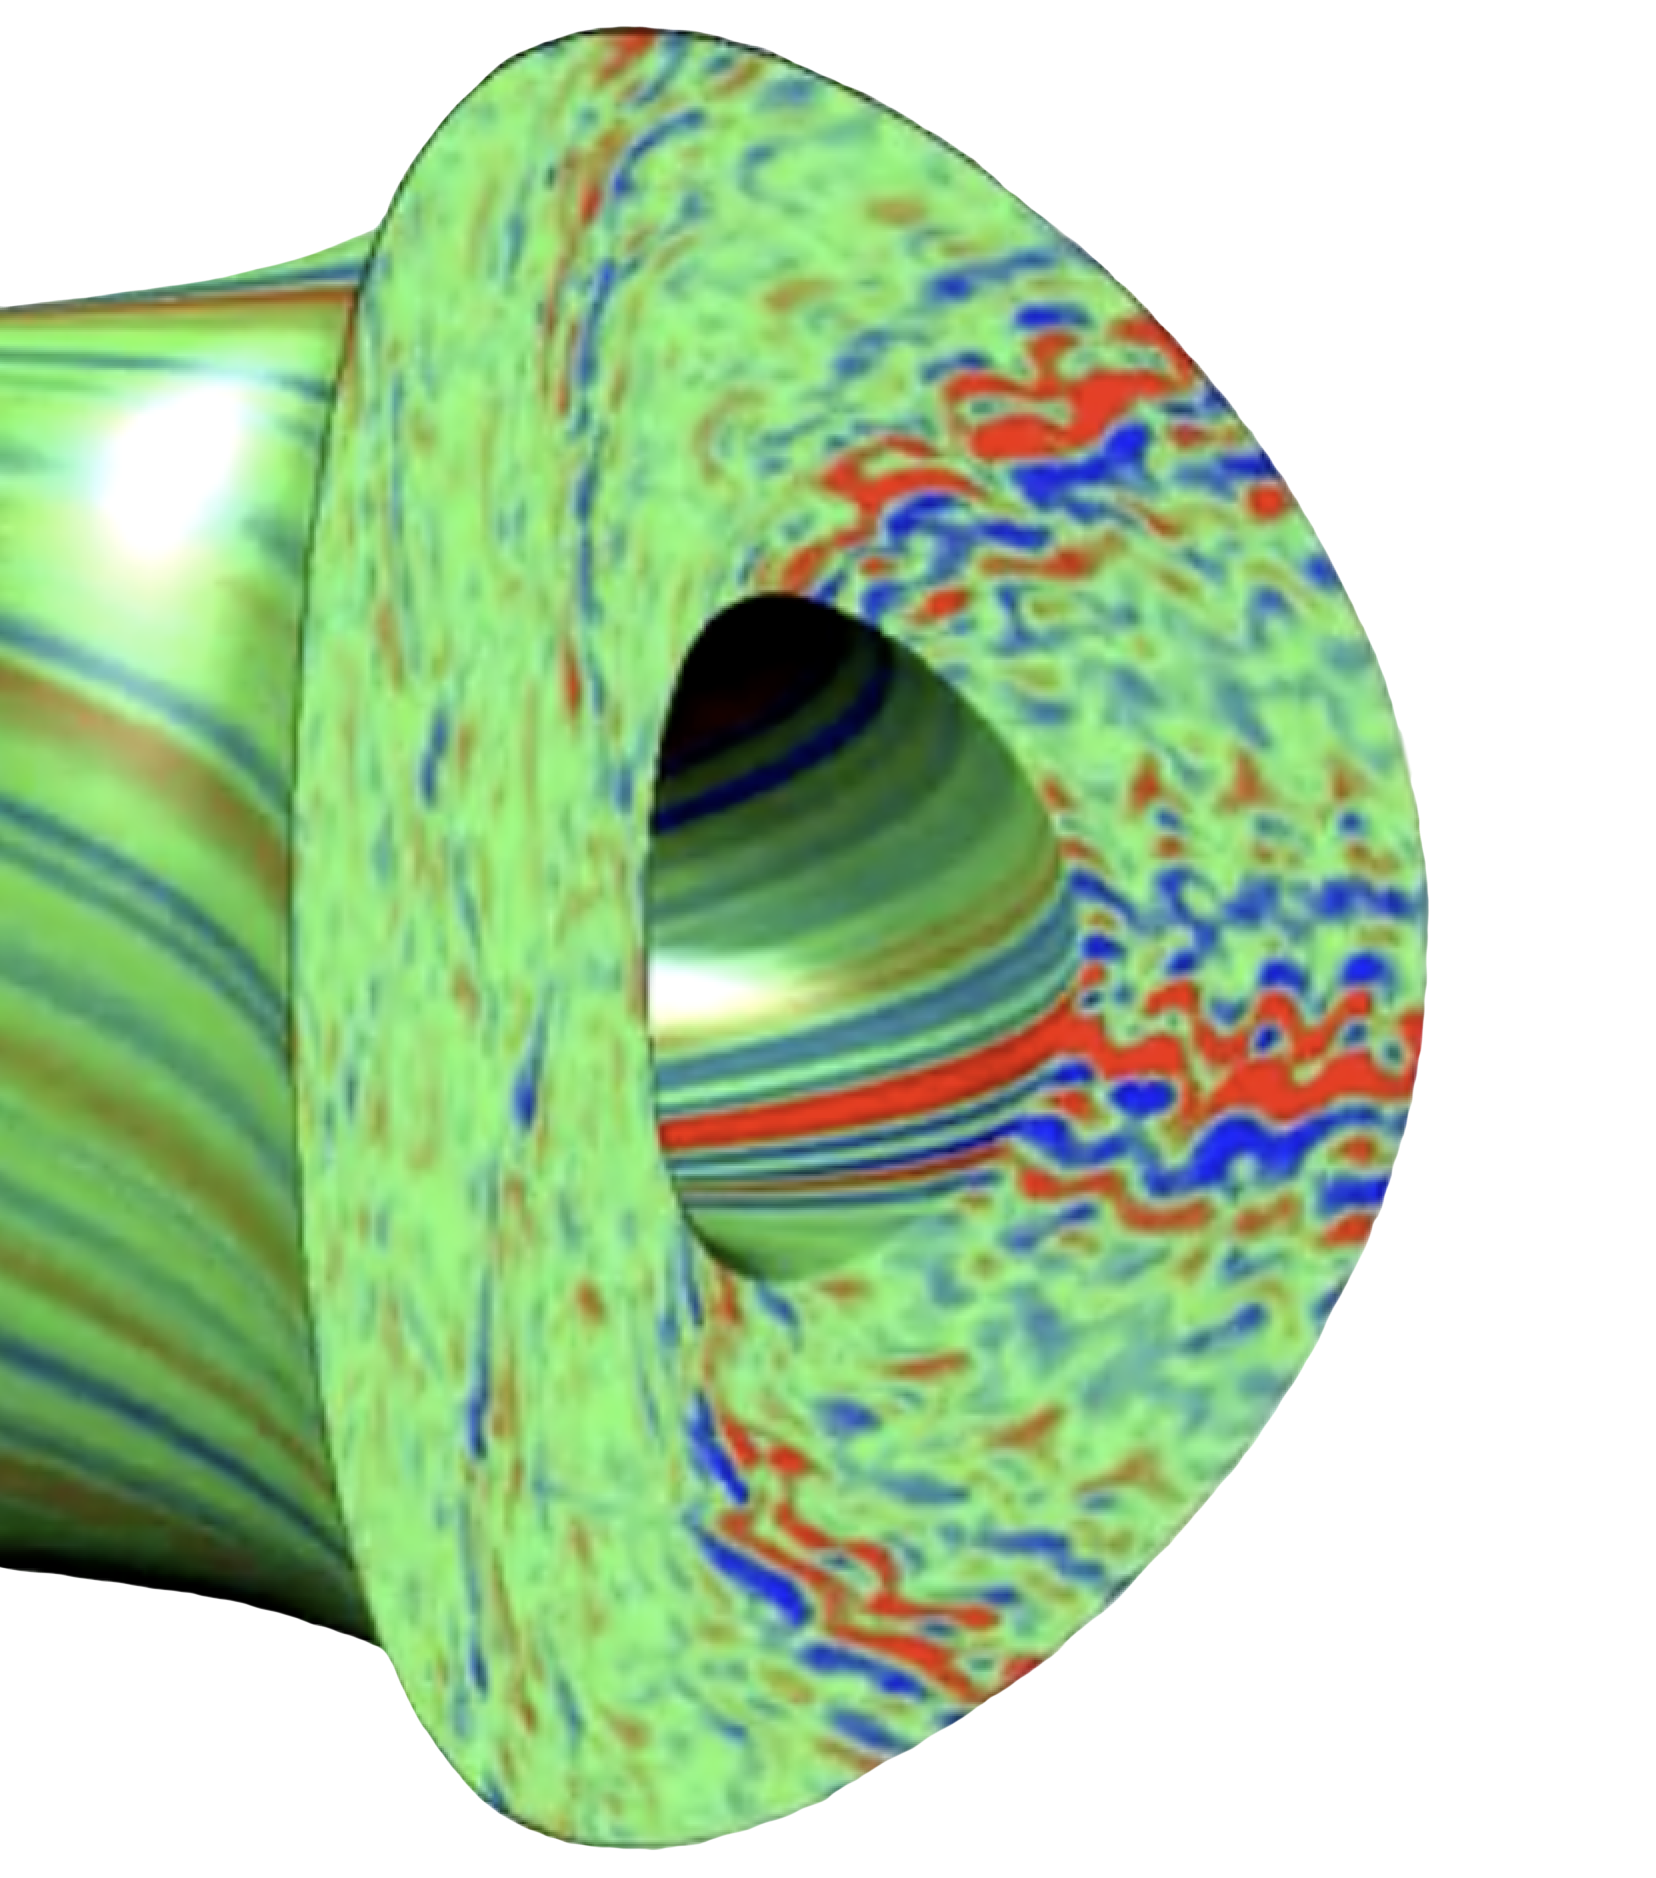
\includegraphics[width=\textwidth]{Presentation/turbulence.png}}
			\end{figure}
			{\tiny Simulation eines Plasmaschlauch von Jeff Candy und Ron Waltz mit Code GYRO}
		\end{minipage}
	\end{frame}

	\section{Turbulenz im Plasma stabilisieren}
	\begin{frame}
		\frametitle{Anpassung der Magnetfeldlinienrichtung}
		Verdrillen der magnetischen Flussdichte $\vect{B}$ überführt Plasma in stabilen Zustand \\[0.2cm]
		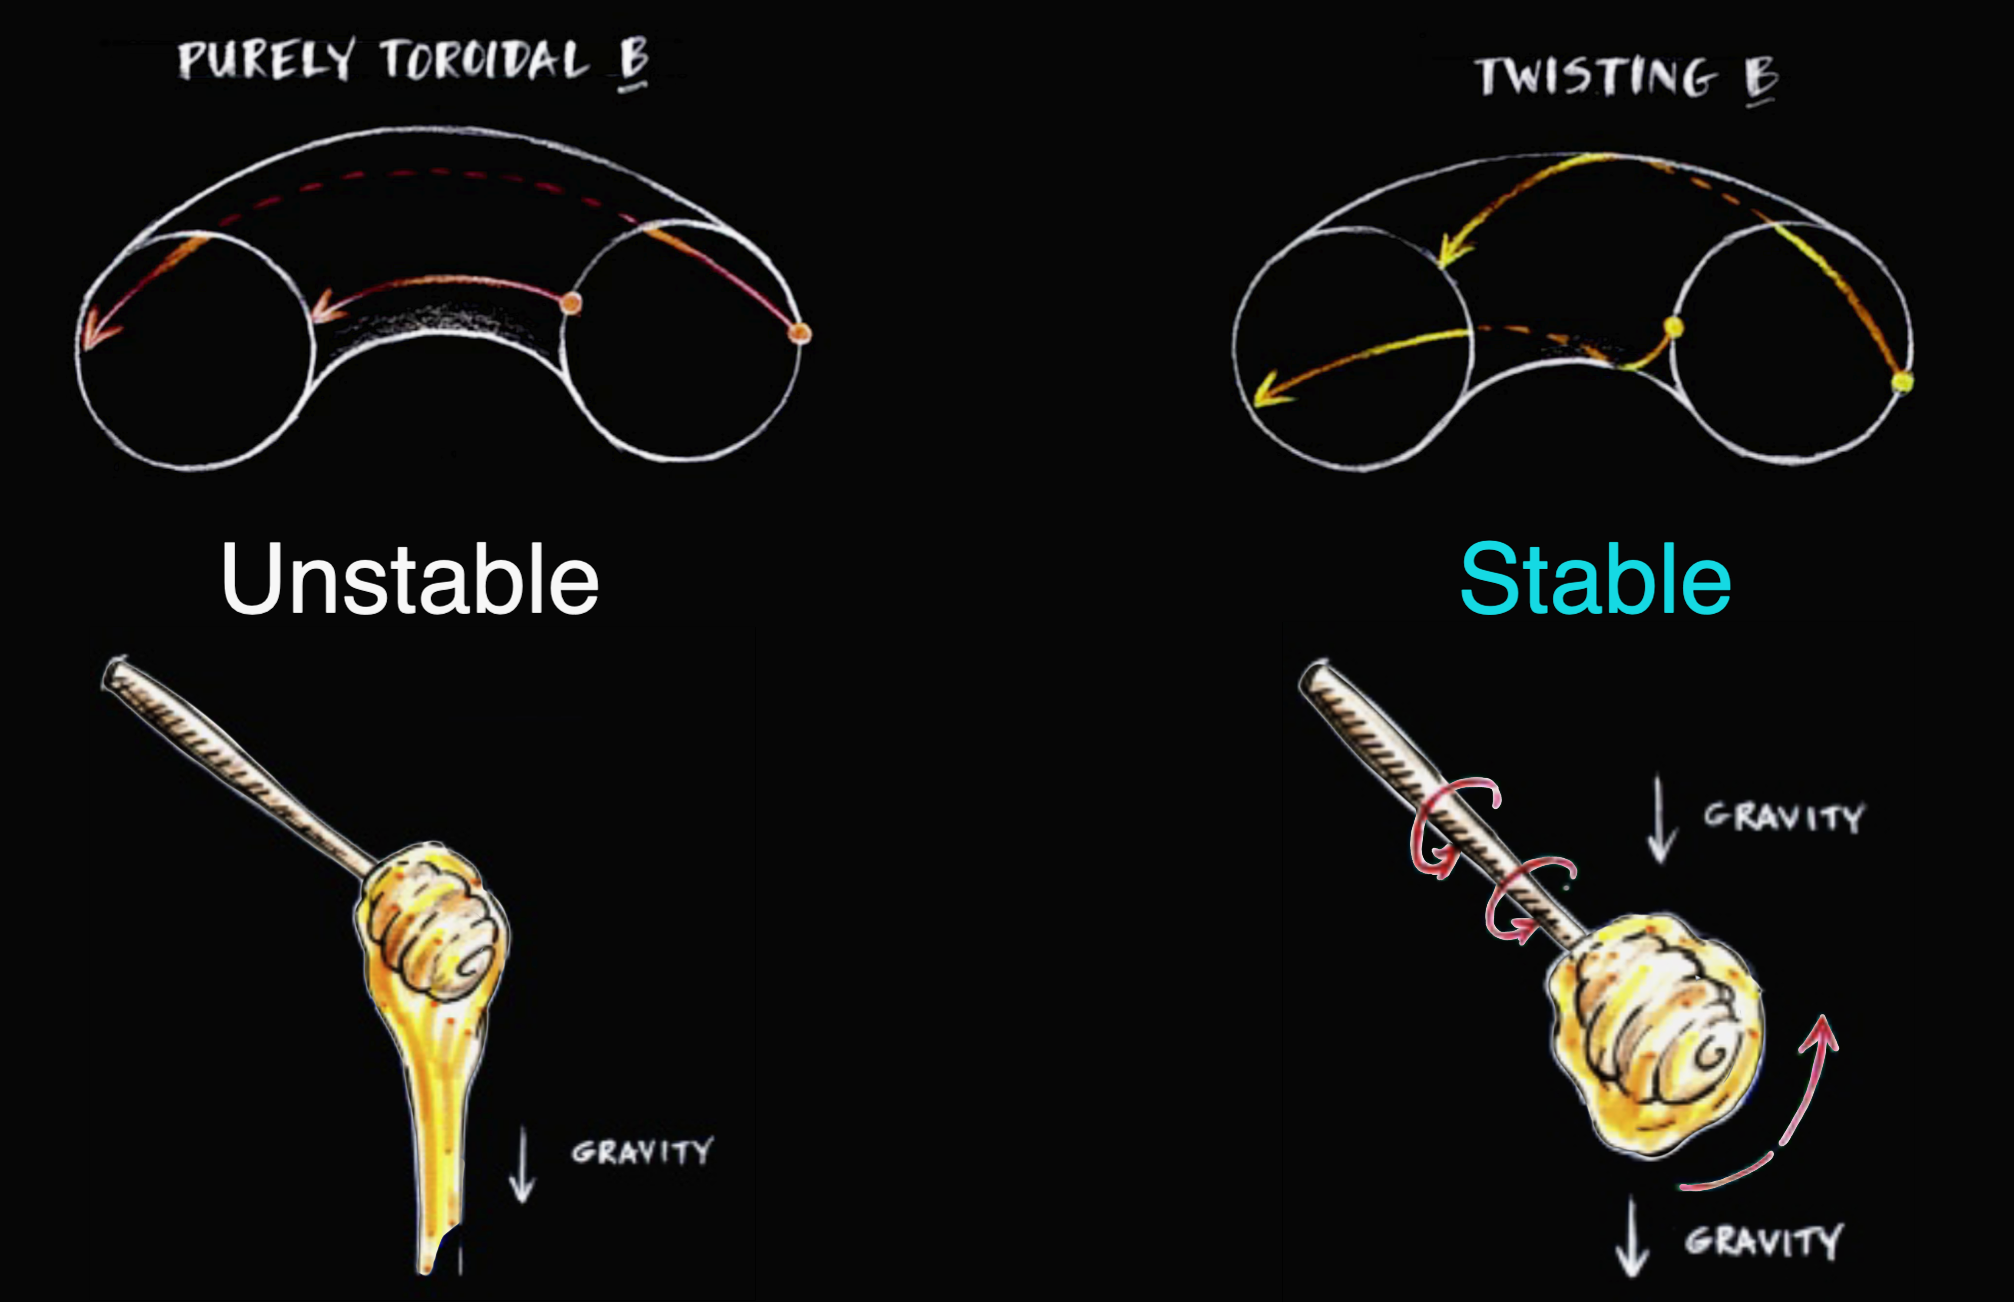
\includegraphics[scale=0.25]{Presentation/Stabilzation_Mechanism_black.png}
	\end{frame}
	
	\begin{frame}
		\frametitle{Turbulenzen verringern}
		\begin{minipage}{0.6\textwidth}\raggedleft
			\begin{itemize}
				\item Wirbelströmung verursachende Partikel folgen meistens Feldlinien
				\item Turbulenzen können mit negativer magnetischen Scherung verringert werden
				\item Verdrehung in Richtung der "Guten Krümmung"
				%\item Umkehrung der magnetischen Scherung verdreht Wirbelströmung in kleinen Abständen in Richtung der "Guten Krümmung"
				%\item Umgekehrte magnetische Scherung wird erzeugt durch Quetschung des Magnetfelds bei hohen Plasmadruck
				\item Durch die Verformung des Plasmas kann sich Scherung lokal verändern
			\end{itemize}
		\end{minipage}
		\begin{minipage}{0.3\textwidth}
			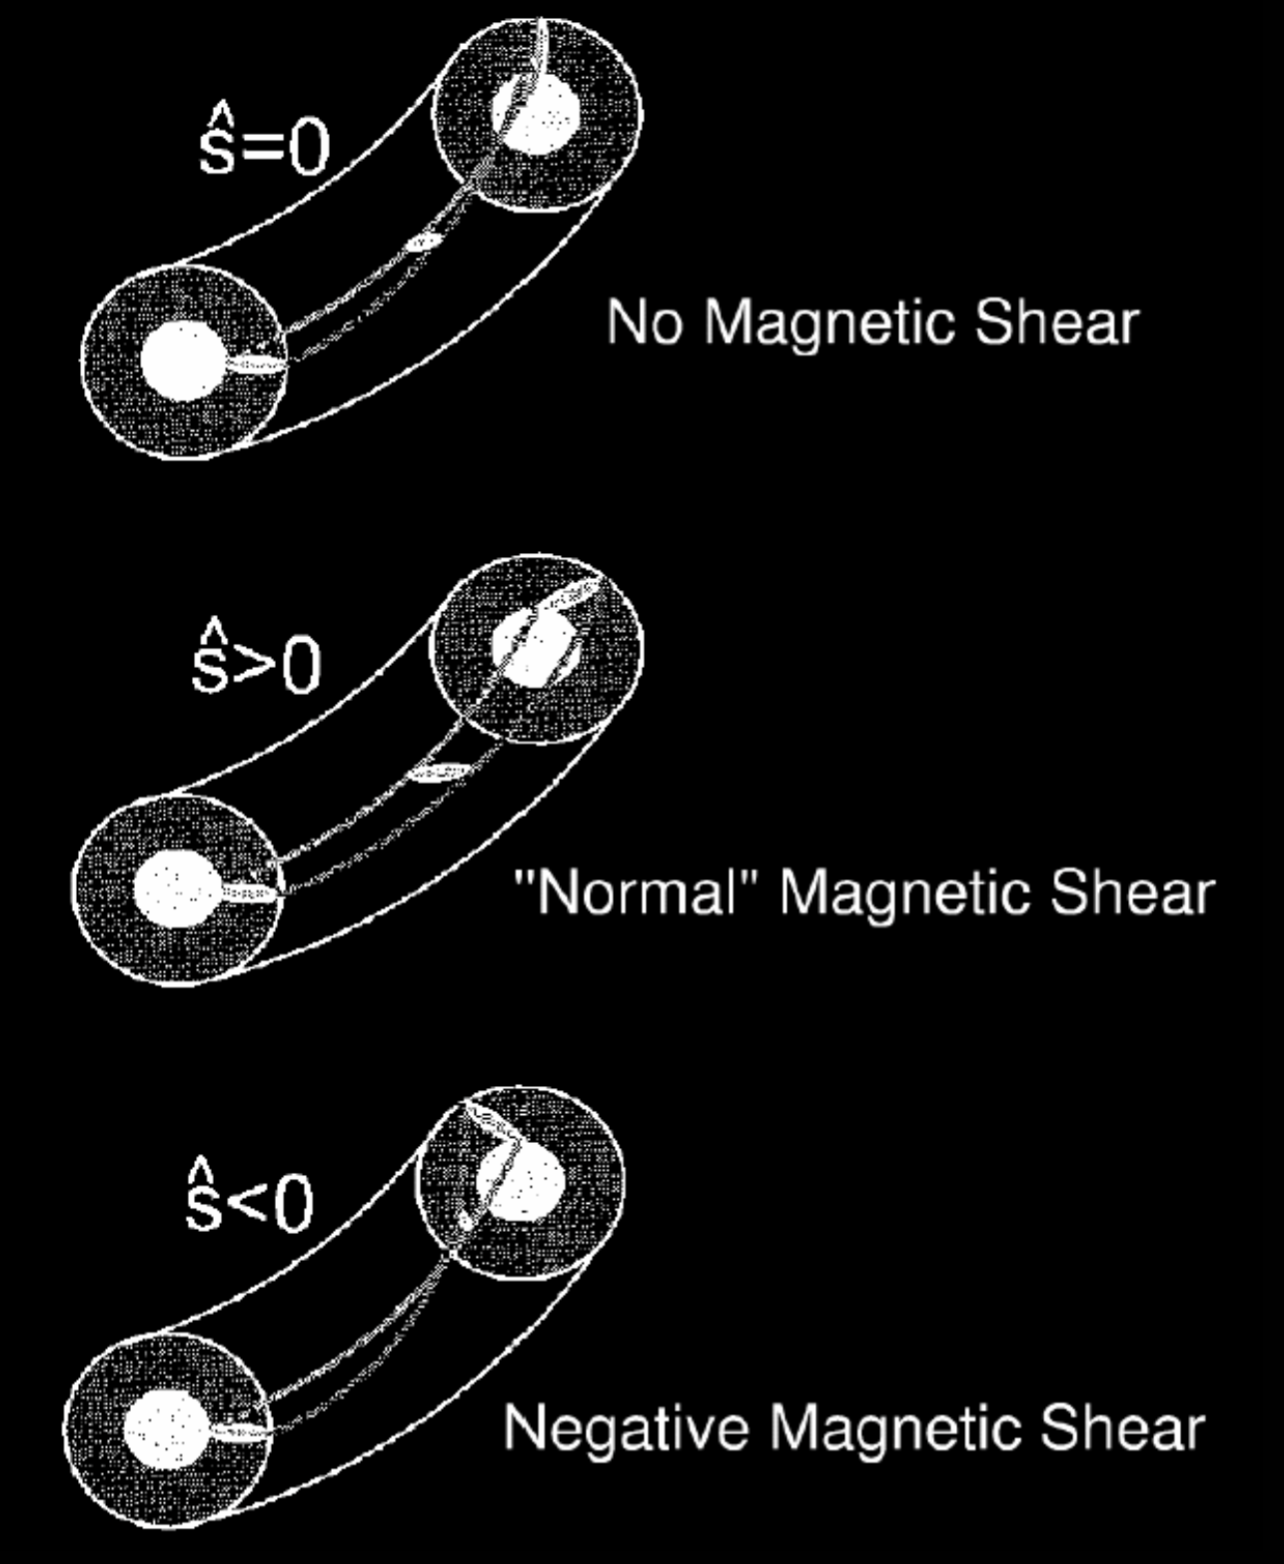
\includegraphics[scale = 0.15]{Presentation/Magnetic_Shear_black.png}
		\end{minipage}
	\end{frame}

	%\begin{frame}
	%	Wirbelströmung, welche größere Längenskalen in \doublequoted{Schlechte Krümmung} transportieren, werden mit Scherung reduziert bis sie sich komplett unterdrücken.
	%	\frametitle{Regelung oder Unterdrückung von Turbulenzen}
	%	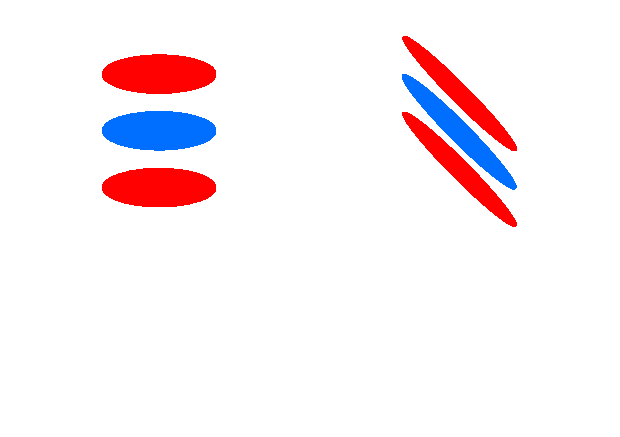
\includegraphics[scale = 1.3]{Presentation/Shearing.pdf}
	%\end{frame}

	\begin{frame}
		\frametitle{Regelung oder Unterdrückung von Turbulenzen}
		{\tiny Waltz, Kerbel, Phys. Plasmas 1994 w/ Hammett, Beer, Dorland, Waltz Gyrofluid Eqs., Numerical Tokamak Project, DoE Computational Grand Challenge}
		\begin{tabular}{c c}
			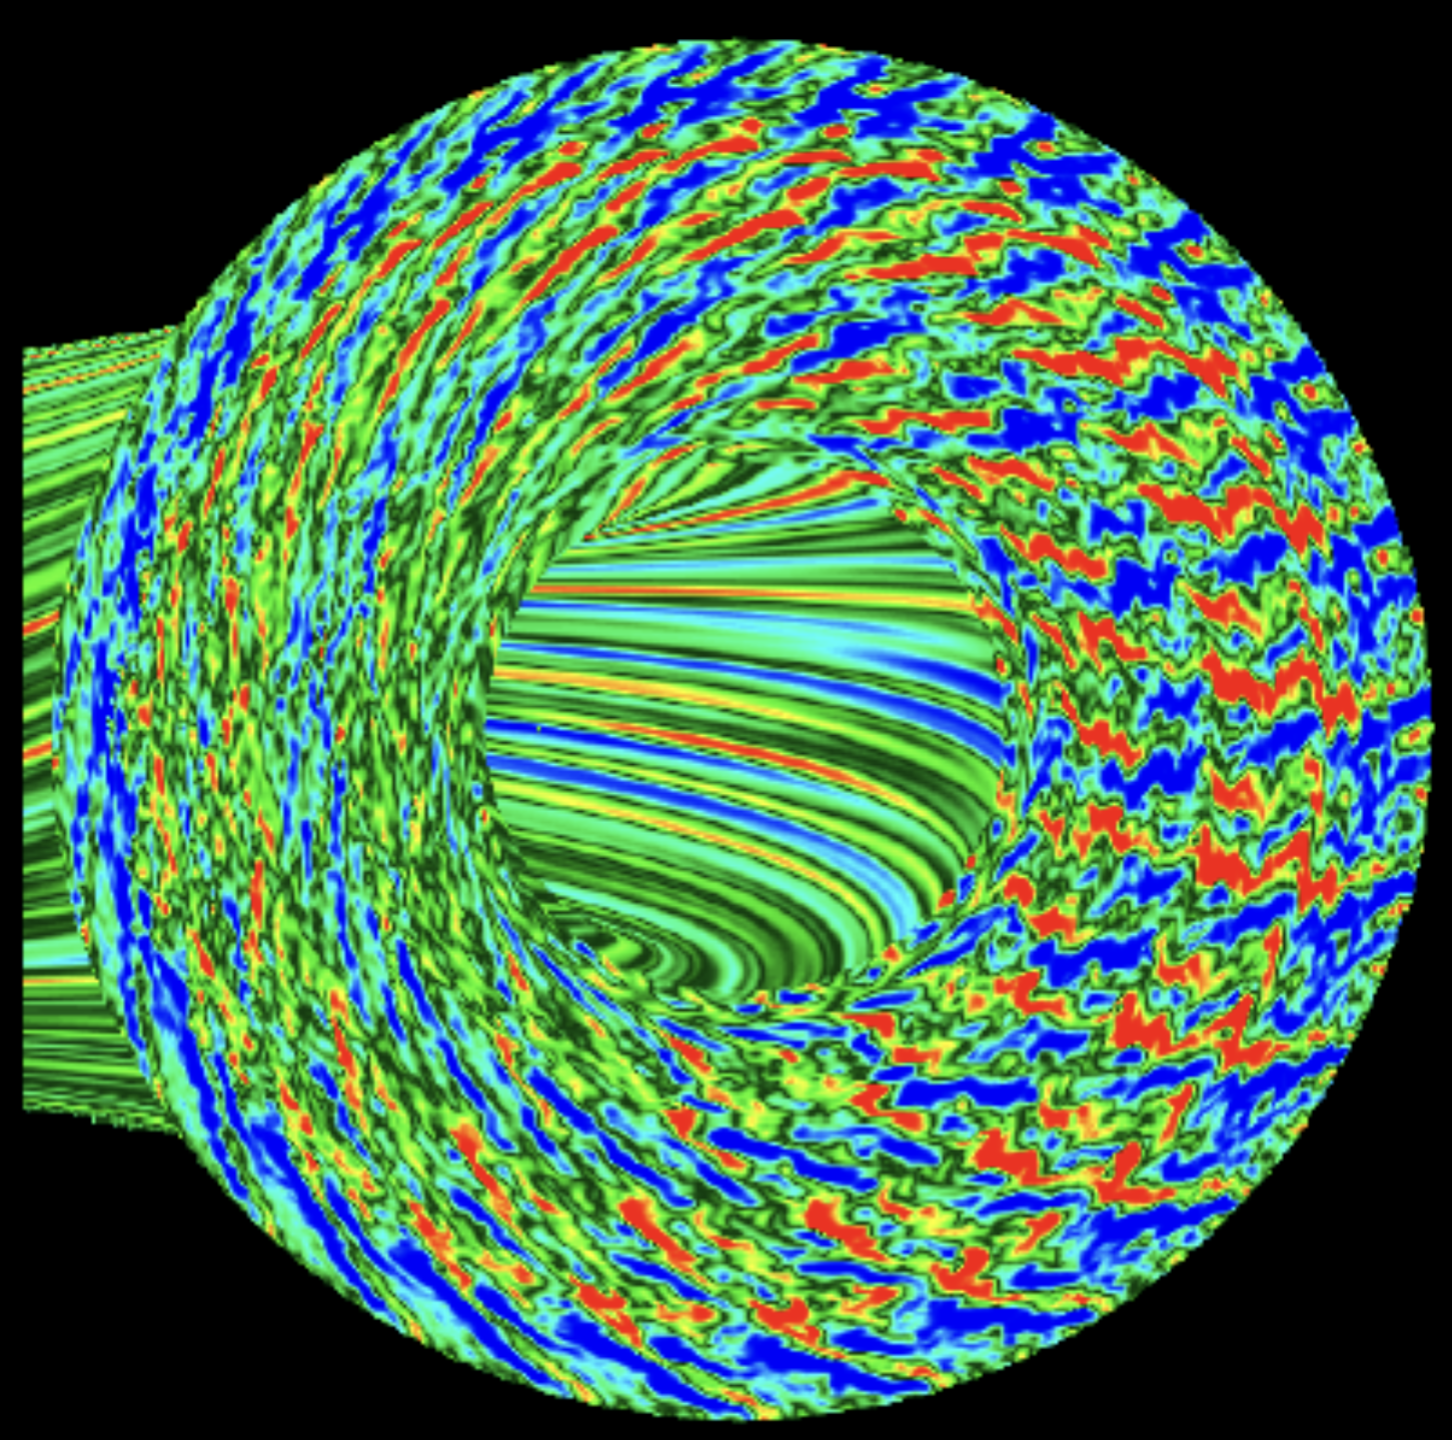
\includegraphics[scale = 0.15]{Presentation/Stablized_Plasma_Interaction.png} & 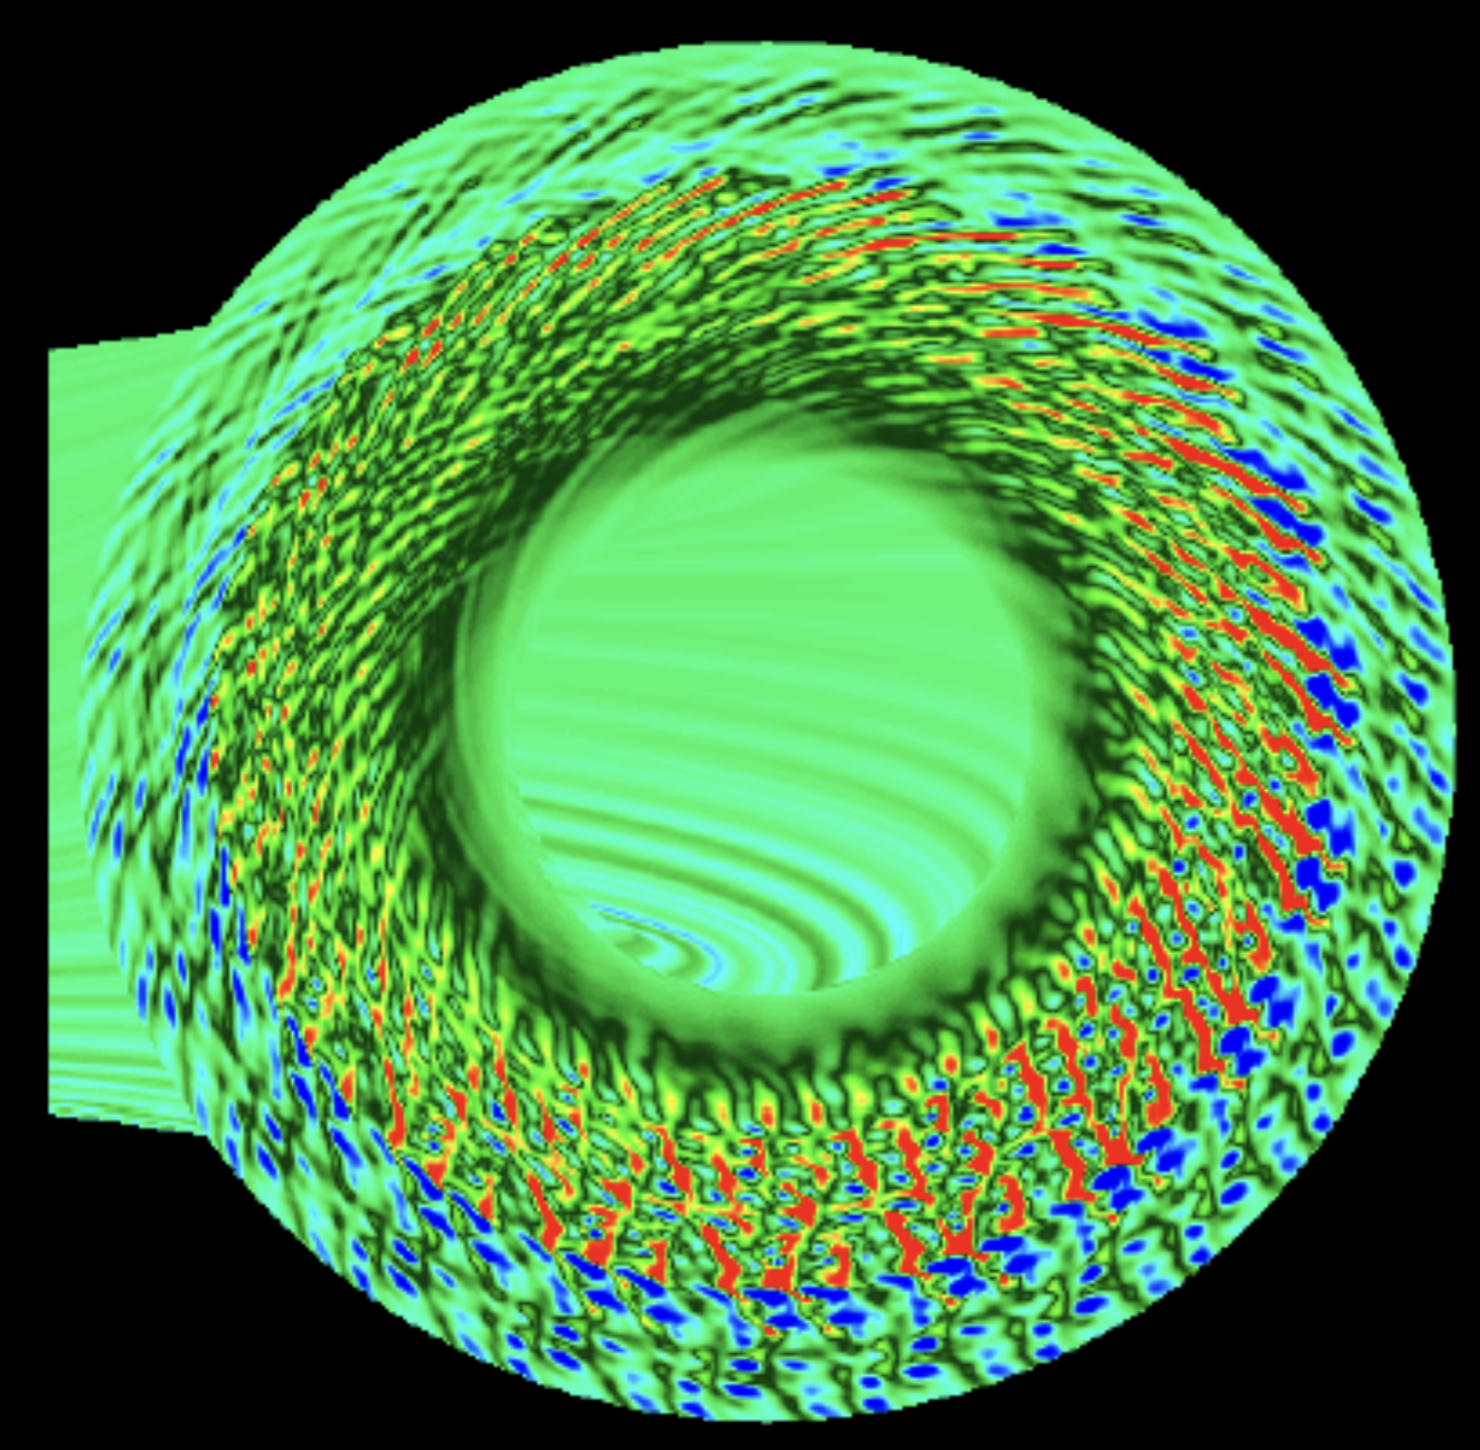
\includegraphics[scale = 0.15]{Presentation/Stablized_Plasma_LongScale.png} \\
			Dominante nichtlineare Interaction  & Zusätzlicher verscherter Zonal Flow \\
			zwischen turbulenter Wirbelströmung & unterdrückt Turbulenz komplett \\
			und kontrollierten Zonal Flow & \\
		\end{tabular}
	\end{frame}

	%\section{Parallelen zur Atmosphären-Physik}
	%\begin{frame}
	%	\frametitle{Zonal Flow auf Jupiter vs. Tokamak Reaktor}	
	%\end{frame}

	\appendix
	\section*{Appendix}
	\begin{frame}
		\frametitle{Danke für die Aufmerksamkeit!}
		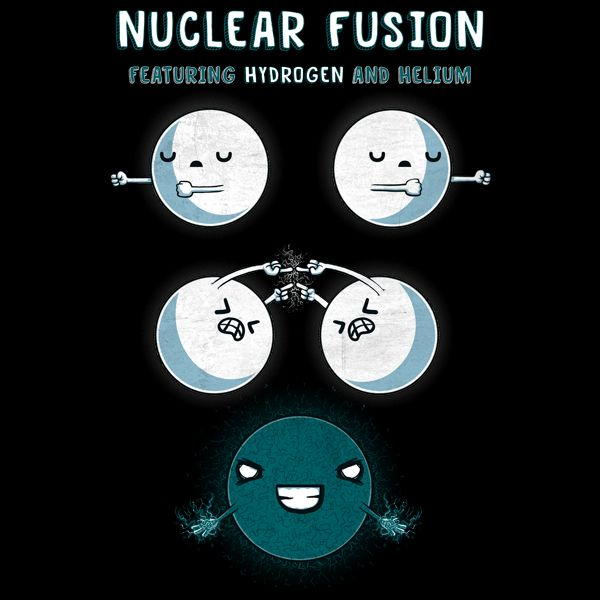
\includegraphics[scale = 0.3]{Presentation/Fusion_Meme.jpeg} \\
	\end{frame}

\end{document}






